
\section{Mocha}

Mocha\footnote{Página oficial de Mocha: http://visionmedia.github.io/mocha/} es un framework Javascripts para realizar pruebas unitarias. Sus creadores lo definen como:

\begin{quote}
\textit{Mocha is a feature-rich JavaScript test framework running on node.js and the browser, making asynchronous testing simple and fun. Mocha tests run serially, allowing for flexible and accurate reporting, while mapping uncaught exceptions to the correct test cases. Hosted on GitHub.}
\end{quote}


Y sinceramente, creo que la definición no puede ser más acertada. Permite crear test con relativa facilidad y con una sintaxis clara y concisa. De puedo decir, que es ''simple, flexible y divertido''\footnote{En la cabecera de su web podemos leer "mocha simple, flexible, fun"}.


\subsection{Características}

Entre sus características más destacables están:


\begin{itemize}
\item \textbf{Soporte para NodeJs.} No sólo soporta el uso con NodeJS sino que esta empaquetado para NPM, por lo que, la instalación y la puesta en marcha resulta muy, muy sencilla. También existen plugins para utilizarlo con GruntJs.
\item \textbf{Soporte para diferentes navegadores.} Por lo que, podemos probar nuestro interfaz en el navegador y verificar su correcto funcionamiento.
\item \textbf{Informes.} Tiene opciones para generar informes en varios formatos dependiendo de las necesidades.
\item \textbf{Uso de cualquier librería de afirmaciones(Assertions).} Existe principalmente cuatro librerías que pueden ser utilizadas con Mocha Chai, Should, Expect y Better-Assert.
\item \textbf{Soporte para test síncronos y asíncronos.} Permite abarcar todas las necesidades de nuestro código.
\end{itemize}

\subsection{Ejemplo}

\begin{wrapfigure}{r}{0.2\textwidth}
  \begin{center}
    
\includegraphics[width=0.2\textwidth]{imagenes/mocha-logo}
  \end{center}
  \caption{Mocha}
	\label{fig:mocha}
\end{wrapfigure}


He aquí un simple ejemplo de uso de mocha. 

\lstinputlisting{recursos/array-test.js}


Para empezar, debe realizar importar la librería de afirmaciones (assertions) que vamos a utilizar en el presente ejemplo se ha utilizado assert\footnote{En MindMapJS se ha utilizado Should y Chai}. 

Las líneas 2 y 3 describen a su vez, un módulo y submódulo de ejecución. En nuestro caso el módulo lo hemos llamado "Array" y el submódulo de ejecución "indexOf()". Conviene ser descriptivos en los nombres de los módulos y submódulos. 

La línea 4 describe una prueba unitaria a la que le asociamos una función anónima con las afirmaciones necesaria.

Una vez escrita la prueba unitaria ejecutamos el siguiente comando “mocha -R *.js” obtenemos el resultado que podemos observar en la figura \ref{fig:mochaejecucion}.

\begin{figure}[htbp]
\centering
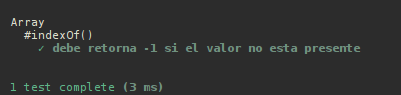
\includegraphics[width=0.6\textwidth]{imagenes/mochaejecucion}
\caption{Resultado de ejecutar mocha -R spec *.js}
\label{fig:mochaejecucion}
\end{figure}

Existe una función especial, que podemos observar en la línea 5 del siguiente código. Esta función especial es "beforeEach", que tiene la misión de ejecutarse antes de cada test unitario. Nuestro ejemplo podemos ver que la hemos utilizado para inicializar variables.

\lstinputlisting{recursos/array1-test.js}

El resultado de ejecutar nuestro nuevo test es.

\begin{figure}[htbp]
\centering
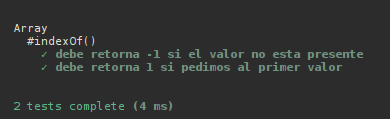
\includegraphics[width=0.6\textwidth]{imagenes/mochaejecucion1}
\caption{Resultado de ejecutar mocha -R spec array1-test.js}
\label{fig:mochaejecucion1}
\end{figure}

Como se puede deducir, de los ejemplos anteriores, Mocha nos proporciona los mecanismos básicos para poder realizar test unitarios fáciles, rápidos y sobre todo sencillos.

